\chapter{Transport mode application to heavy-flavor evolution}
In this chapter, we shall start to focus on applying the LIDO transport model to the heavy-flavor section, and discuss in detail how a transport model fits into the complex dynamics that heavy flavor particles undergoes in the heavy-ion collision environment.

Heavy flavor is a charming probe for the medium created in heavy-ion collisions. 
Its large mass guarantees an negligible thermal production contribution at least for present LHC top beam energies for heavy-ion program (there are estimates that thermal contribution can play a row in future FCC collider).
Therefore, heavy flavors are almost always created in initial hard processes. 
By hard processes, it includes both the hardest few body collisions, as well as the associated high-virtuality parton evolution.
Their dilute population also suppresses the chances that they annihilates against their anti-particles during the medium evolution.
As a result, heavy flavors are created at relatively early stages of the heavy-ion collision and experienced the entire medium evolution and encodes valuable information about the medium.
On the theory side heavy flavor has a rich variety of physics interests. 
At high $p_T$, the evolution of heavy flavor particles merges into the context of jet dynamics and jet energy loss study; at intermediate $p_T$ the mass hierarchy predicted for the medium modifications;
and low $p_T$, heavy flavor is one of the key messengers for the thermalization processes inside QGP due to its long relaxation time compared to light partons.
On the experimental side, their unique flavors, masses, and decay modes also give us the chance to reconstruct heavy flavor (heavy meson / baryon) observables directly.

There are two types of heavy quarks that are most relevant for nowadays hard-probes study, the charm quark with mass $1.3$ GeV, and the bottom quark with mass $4.2$ GeV.
The reason top quark ($173$ GeV) is out of our discussion is due to its extremely short life time ($\sim 5\times 10^{-25} \approx 0.15$  fm/$c$ in the rest frame) so it barely interacts with the QGP before it decays predominantly into bottom quarks.
Even though there has also been proposal for taking advantage of this short time scale to probe the temporal structure of the QGP in its early stages, we shall focus on the charm and bottom flavor in this thesis.

To build a comprehensive simulation framework for the fate of heavy quarks in relativistic heavy-ion collisions requires a multi-component and multi-stage modeling.
Here we summarize this simulation framework in the following flow chart as a guide line for this section, figure \ref{fig:flowchart}.

\begin{figure}
\centering
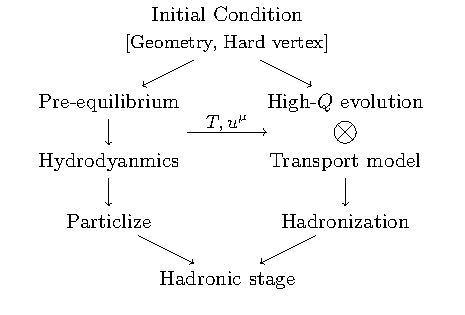
\includegraphics[width=.8\textwidth]{flowchart.pdf}
\caption{hh}
\label{fig:flowchart}
\end{figure}

In the previous two chapters, we have introduced the left branch of this flow chart, which is a relativistic viscous hydrodynamics based simulation for the bulk medium evolution.
The right branch is a model for the hard parton (heavy flavor) evolution.
The heavy quarks are produced in hard processes.
The hard processes contains both the hard matrix-element as well as the virtuality evolution of the parton (the DGLAP evolution or termed vacuum-like evolution).
One complication in the presence of medium, one complication is that vacuum-like evolution starts to occupied the same space-time of the medium induced processes at low-virtuality.
And should one interfaces the two calculations is still an interesting topic under debate.
One of the many obstacles is that multiple emissions / branchings are treated very differently in the two calculations.
For the vacuum-like evolution, the evolution variable is the virtuality scale with the space-time information integrated out, while the transport model evolves the systems in time, with virtuality integrated out below a certain scale.
There are many recent progress in both theory developments and newly design event-generators to solve this problem.
In this chapter, we shall focus on one possible solution to interface the two in section 1.
The in medium propagation of parton requires the medium properties as input. 
To zeros order of approximation, we specify the medium with its flow velocity and the equilibrium temperature, although the viscous hydro provides far more off-equilibrium information. 
This is discussed in section 2.
The heavy flavor hadronization model is introduced in section 3, which is a previously developed model that interpolates high-$p_T$ fragmentation processes and low-$p_T$ in medium recombination production of heavy hadrons.
Finally, in section 4, we also briefly introduced how this simulation framework of open heavy flavor can be coupled to the quarkonium evolution, but for more details, please refers to the thesis work [].

\section{Initial production of heavy flavor}
The initial hard processes are computed using perturbative QCD based or related Monte-Carlo event generator.
The general set up for such a computation in proton-proton collision is the factorization theorem \ref{fig:factorization}.
Where the perturbative QCD calculation provides the physics at short distance (a hard scale $Q^2$): the partonic matrix-elements $\hat{\sigma}_{ij\rightarrow kl}$.
The partonic configuration inside the proton characterized by the parton-distribution function (PDF) and the hadronization of the final state parton into hadrons are non-perturbative inputs.
Although these non-perturbative objects general cannot be computed from first principal and has to be extracted from measurements, their scale evolution in $Q^2$ can be described in perturbative QCD, knowns as the DGLAP evolution equations.
This scale dependence comes from that the exclusive process  $i+j \rightarrow k+l$ described by the fixed order matrix-elements is always modified by the parton branching and virtual correction that is of order $\alpha_s \ln Q^2/\mu^2$.
These corrections takes into account the fact that the initial high-virtuality parton $i$ (or $j$) may also come from a splitting processes of low virtuality parton $i'$ (or $j'$) from the proton, including virtually correction. 
Similarly, the final state high virtuality parton $k$ (or $l$) may also splits into a low virtuality parton $k'$ (or $l'$) before it becomes a hadron, including virtual correction.
The same argument also applies to partons $i', j', k', l'$. 
Eventually, one gets a series of contribution where although each term contains an additional power of $\alpha_s$, but is magnified by $\ln Q^2/\mu^2$ if there is a large gap between the hard scale $Q^2$ and the PDF scale $\mu^2$ at which it is measured.
The DGLAP evolution equations resum these logarithmic contributions systematically to increase the predictive power of the perturbative calculation of the inclusive cross-section.
Moreover, a useful parton-shower picture can be built from the process and with a probabilistic interpretation and Monte Carlo technique, one can mimic the exclusive final states from these sequences of parton branching processes.

In our studies, we have tried to use both inclusive cross-section program as well as Monte-Carlo event generator to initialize the heavy quark production.
Next we will explain their merits and draw backs for our purposes.

\paragraph{Initialize from inclusive cross-section program}
We use FONLL (Fixed Order Next to Leading Log) to generate the inclusive production cross-section of heavy flavor at partonic level.
The FONLL program is a combination of the fixed order (NLO) massive matrix-elements and a massless resummation program.
It predicts the single inclusive differential cross-section $d^2\sigma/dydp_T$. 
Then, one can sample the initial heavy quark's momentum from this differential cross-section.
The advantages are
\begin{itemize}
\item[1.] Sampling / weighting the inclusive cross-section is fast.
\item[2.] Provide interface to nuclear PDFs.
\item[3.] First principal approach for proton-proton collision.
\end{itemize} 
However, there are also disadvantages, 
\begin{itemize}
\item[1.] It only predicts single particle distribution and one cannot initialize the correlation of the $Q-\bar{Q}$ pair. This is not a problem for open heavy flavor observables, but would be a problem for quarkonium study.
\item[2.] The space-time picture of the production process is lost. One do not know whether the virtuality evolution takes a finite amount of time. So we have to assume charms quarks are produced at proper time $t=0^{+}$, which is always before the in-medium transport. But later we will see that from event generator simulations, the evolution can take a finite amount of time, overlapping with the QGP evolution.
\item[3.] Lacking the exclusive final state. Again, it is not a problem for open-heavy flavor study. But to describe full jets, one really needs an exclusive partonic final state of the virtuality evolution to initilize the partonic transport model.
\end{itemize}

\paragraph{Initialize from Monte-Carlo event generator.}
\begin{figure}
\centering
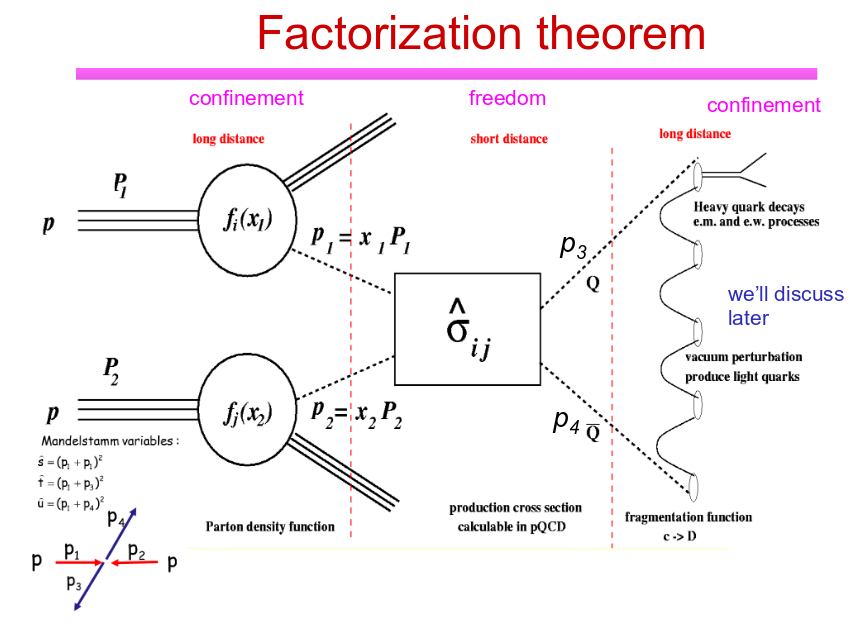
\includegraphics[width=\textwidth]{factorization.png}
\caption{
%https://indico.cern.ch/event/680421/contributions/3096162/attachments/1697092/2731944/J.Huston_Introduction_to_QCD_from_an_LHC_perspective-02.pdf
}
\label{fig:factorization}
\end{figure}

Another approach to generate initial hard process is to use high energy Monte-Carlo event generator, such as Pythia [].
Pythia implements the leading order (LO) matrix-elements for hard QCD processes, including LO production of heavy flavor particles,
$g+g\rightarrow Q+\bar{Q}$ and $q+\bar{q}\rightarrow Q+\bar{Q}$.
A parton shower will be generated based on the hard processes.
In fact, in high energy collisions, the LO production of heavy flavor is only a fraction of the total heavy flavor cross-section, the rest of them are created in the parton showers from the so-called gluon splitting and flavor creation processes.
The former corresponds to a situation where the heavy flavor pair comes from a final state gluon splitting; and the latter produces the pair in initial state gluon splitting and is put-on shell by the hard scattering.
These contributions also mimic certain pair correlations with non back-to-back angular correlations.

The disadvantage is of course the event generator is not a first principal computation of the heavy flavor production.
However, there are many benefits of having an exclusive final state.
\begin{itemize}
\item Although the parton shower is evolved as a function of virtuality $Q^2$. A qualitative space-time picture can be built by measuring the formation time of each branching by $2x(1-x)E/k_\perp^2$. In this way, we will see that the vacuum radiation off a heavy quark can last for a long time.
\item With the space-time picture, it is easier to analyze what kind of vacuum branchings should be modified in the presence of a medium.
\item Can be used to initialize the full transport model to study jets. 
\end{itemize}

\paragraph{Heavy flavor production baseline} In the course of our study, we used both the FONLL program and the Pythia event generator to initialize the momentum space. 
It is important to check that first whether they predict similar heavy flavor production in nuclear collisions and proton-proton collisions, and second if they provide good descriptions of the experimental measurement in proton-proton collisions.
In the upper plot of figure \ref{fig:pythia-fonll}, we compare the $p_T$ differential cross-section of $p+p\rightarrow c$ from FONLL calculations (lines) and from Pythia simulations (symbols), and for Pb+Pb collision (red) and p+p collision (blue) at the LHC energy $\sqrt{s}=5.02$ TeV.
For p+p system, we use the CT10 parton distribution function and for Pb+Pb system, the nuclear modification to the parton distribution is using the EPS09 parametrizaiton.

We note that the absolute value of the cross-sections are different.
Fortunately, the observables that we are interested in nuclear collisions are always ratios such as the nuclear modification factor $R_{AA}$, and the momentum-space anisotropy of heavy meson $v_n$ which is dimensional less. 
Therefore the shape of the spectra is the key feature we would like to compare between the two calculation and we have rescaled the FONLL curve.
We see that their shapes are very similar.
When calculation $R_{AA}$, we are dividing the cross-section from nuclear collision to that of the proton-proton collision.
To see how much the modulation in $R_{AA}$ is contributed by the nuclear PDF effects, we take the ratio between the AA and pp results in the upper plots to get an ``$R_{AA}$" for the nuclear PDF effects in the bottom plots.
We can see that FONLL and Pythia simulation predicts consistent modulation: the initial production AA spectra of charm quark at low-$p_T$ is suppressed compared to the pp spectra, due to the shadowing effect of the small-$x$ gluon. 
At higher $p_T$, the ratio increase and slightly shoots over  unity, this is because the there is an anti-shadowing region of the gluon at larger-$x$.

\begin{figure}
\centering
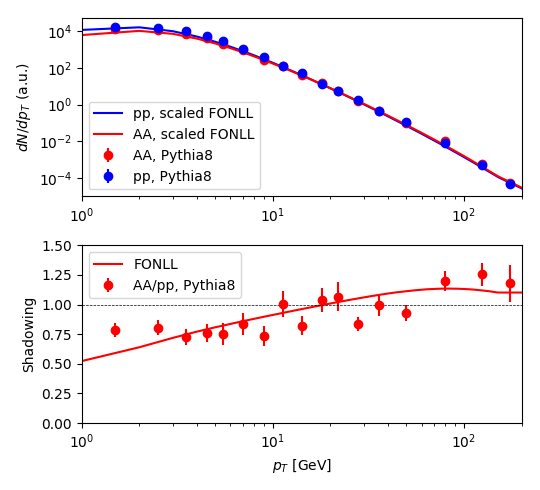
\includegraphics[width=.8\textwidth]{pythia-vs-fonll.png}
\caption{}
\label{fig:pythia-fonll}
\end{figure}

\section{Interfacing vacuum shower with in-medium transport}
Interfacing the vacuum shower that evolves with virtuality and the transport equation that evolves with time is a difficult task. 
We shall provide a reasoning for the prescription we use following some of the recent developments [].
Start by considering a splitting of a hard parton which is created at the boundary of a brick medium.
This splitting has a formation time depending on its transverse momentum (or virtuality) $\tau_f \sim 2x(1-x)E/k_\perp^2$.
It is very likely that the radiated gluon (or the quark) interacts with a scattering center in the medium, denoted by the crossed circle.
If the virtuality of the splitting is very large, then the formation time is small.
The argument is that scatterings at time $t$ that is well separated from the formation time $\tau_f \ll t$ are independently from the initial vacuum-like splitting process; while scatterings within $\tau_f$ can change the branching probability.
So, we determine whether the vacuum branching should be modified in medium by the number of scatterings before $\tau_f$.

\begin{itemize}
\item For a branching with large virtuality (left of figure \ref{fig:vac-med-interface}) that $N = \tau_f/\lambda \ll 1$ (translates into $k_\perp^2 \gg \alpha_s  \omega T$). 
There chance for the medium interaction to modify the vacuum branching is negligible.
\item Hold the energy of the radiaion, while decrease its transverse momentum (middle of figure \ref{fig:vac-med-interface}) so that $N = \tau_f/\lambda \lesssim 1$ ($k_\perp^2 \gtrsim \alpha_s  \omega T$). 
Now, there is order one scatterings with the medium. 
The transverse momentum of the gluon is modified a little but still dominated by the initial virtuality.
The probability for the branching should also be modified.
For example, a higher twist expansion in terms of $1/k_\perp^2$ takes into account the effect of one interaction with the medium.
\item Further decreasing the initial virtuality of the branching (right of figure \ref{fig:vac-med-interface}) until $N = \tau_f/\lambda \gg 1$.
Now the final transverse momentum has to be determined self-consistently to be $k_\perp^2 \sim \sqrt{\hat{q}\omega} \sim \alpha_s\sqrt{\omega T^3}$. 
When this happens, the initial virtuality of the splitting is completely dominated by the medium effects (a medium scale at $\sqrt{\hat{q}\omega}$). 
And the branching probability should be replaced by a medium-induced calculation.
\end{itemize}
Summarizing the two extreme regions:
Vacuum branchings with $k_\perp^2 \gg \alpha_s \omega T$ is not modified, while branchings with $k_\perp^2 \sim \sqrt{\hat{q}\omega}$ should be treated as medium-induced process instead of vacuum radiation.
It is therefore natural to use $k_\perp^2$ and the fraction of $k_\perp^2$ that is contributed by the medium broadening $\Delta k_\perp^2$ to separate the medium-induced radiation and the vacuum-like radiation.
Since medium induced radiations treated by the transport equation always have $k_\perp^2 = \Delta k_\perp^2$,  our interfacing prescription is then to simply cut-out the vacuum branchings generated by Pythia in the region $k_\perp^2 <  \Delta k_\perp^2$ (this is also known as the vetoed region in the literature).

\begin{table}[h]
\centering
\caption{Treating Pythia branchings inside the medium}
\begin{tabular}{ccc}
\hline
\multirow{2}{*}{Formed inside medium} & $k_\perp^2 > C \Delta k_\perp^2$ & Unmodified\\
 & $k_\perp^2 < C \Delta k_\perp^2$ & Removed\\
Formed outside medium & Unmodified & \\
\hline
\end{tabular}
\label{tab:med-vac}
\end{table}

Since we are interested in heavy quarks,


\begin{figure}
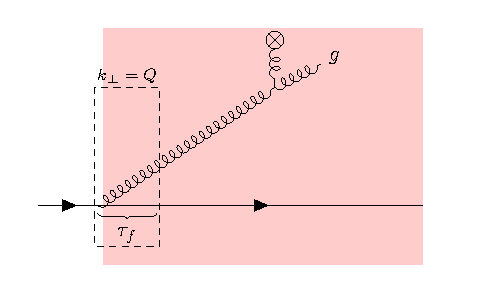
\includegraphics[width=.35\textwidth]{largeQ.pdf}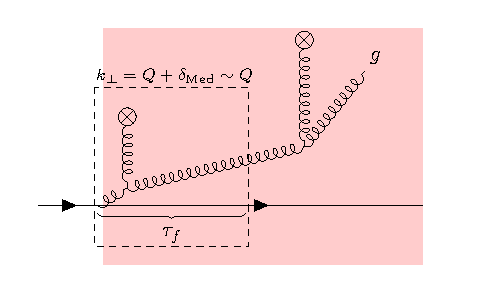
\includegraphics[width=.35\textwidth]{mediumQ.pdf}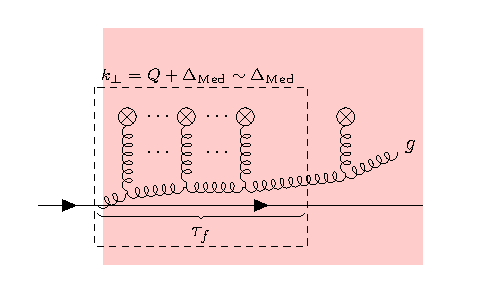
\includegraphics[width=.35\textwidth]{smallQ.pdf}
\caption{}
\label{fig:vac-med-interface}
\end{figure}


\section{Coupling transport dynamics to an evolving medium}

\section{Heavy-flavor hadronization and hadronic stage}

\section{Coupling open-heavy flavor to quarkonium evolution}
